\documentclass[11pt,letterpaper]{article}
\usepackage{rotating}
\usepackage{acl2016}
\usepackage{times}
\usepackage{url}
\usepackage{amsmath}
\usepackage{amsthm}
\usepackage{amsfonts}
\usepackage{latexsym}
\usepackage{graphicx}
\usepackage{appendix}
\usepackage{booktabs}
\usepackage[small]{caption}
\usepackage{subcaption}
\usepackage{xspace}
\usepackage{multirow}
\usepackage{rotating}

\usepackage[inline,shortlabels]{enumitem}
\setlist*[enumerate,1]{label=$(\arabic*)$}
\setlist*[itemize,1]{label=$\bullet$}

\usepackage[T1]{fontenc}
\usepackage[utf8]{inputenc}
\usepackage{amsmath,amssymb}
\usepackage[russian,english]{babel}

\usepackage{cleveref}
\crefname{section}{§}{§§}
\Crefname{section}{§}{§§}
\crefname{figure}{Fig}{}
\crefname{algorithm}{Alg.}{}
\crefformat{section}{§#2#1#3}  % remove space between section symbol and the number


\long\def\devour#1{\ignorespaces}

\renewcommand{\vec}{\boldsymbol}   % optional
\newcommand{\vf}{{\vec{f}}}
\newcommand{\vg}{{\vec{g}}}
\newcommand{\vh}{{\vec{h}}}
\newcommand{\vx}{{\vec{x}}}
\newcommand{\vz}{{\vec{z}}}
\newcommand{\vm}{{\vec{m}}}
\newcommand{\vw}{{\vec{w}}}
\newcommand{\vc}{{\vec{c}}}
\newcommand{\vy}{{\vec{y}}}
\newcommand{\vl}{{\vec{l}}}
\newcommand{\vs}{{\vec{s}}}
\newcommand{\vphi}{{\vec{\phi}}}
\newcommand{\valpha}{{\vec{\alpha}}}
\newcommand{\vxi}{{\vec{\xi}}}

\newcommand{\vmu}{{\vec{\mu}}}
\newcommand{\vtheta}{{\vec{\theta}}}
\newcommand{\veta}{{\vec{\eta}}}
\newcommand{\vomega}{{\vec{\omega}}}
\newcommand{\vpsi}{{\vec{\psi}}}
\newcommand{\vbeta}{{\vec{\beta}}}

\newcommand{\dirac}[2]{\delta_{#1}\left(#2\right)}
\newcommand{\Discrete}{\ensuremath{\mathrm{Discrete}}}
\newcommand{\Dirichlet}{\ensuremath{\mathrm{Dirichlet}}}

\newcommand{\DR}{\ensuremath{\textrm{DR}}}
\newcommand{\model}{\ensuremath{(model)}}
\newcommand{\DRmodel}{\ensuremath{\DR^{\model}}}
\newcommand{\DRlem}{\ensuremath{\DR^{(lem)}}}
\newcommand{\DRnonlem}{\ensuremath{\DR^{(non-lem)}}}

% reduce space before \paragraph command -- http://tex.stackexchange.com/questions/219676/how-to-change-spacing-before-and-after-paragraph-command/219677#219677
%\makeatletter
%\renewcommand\paragraph{\@startsection{paragraph}{4}{\z@}%
%                                    {3.25ex \@plus1ex \@minus.2ex}%
%                                    {-1em}%
%                                    {\normalfont\normalsize\bfseries}}
%\makeatother

\usepackage{amssymb}
\DeclareMathOperator*{\Expect}{\mathop{\mathbb{E}}}
\DeclareMathOperator*{\argmax}{\mathop{\text{argmax}}}


% new math commands

\usepackage{color}
\usepackage{xcolor}
\definecolor{darkgrey}{rgb}{0.2,0.2,0.2}
\definecolor{grey}{rgb}{0.9,0.9,0.9}
\definecolor{darkblue}{rgb}{0.0,0.0,0.5}
\definecolor{darkpurple}{rgb}{0.4,0.0,0.4}
\definecolor{darkred}{rgb}{0.5,0.0,0.0}
\definecolor{darkorange}{rgb}{0.5,0.45,0.4}
\definecolor{darkgreen}{rgb}{0.0,0.5,0.0}
\definecolor{darkergreen}{rgb}{0.0,0.4,0.0}
\definecolor{lightblue}{rgb}{0.8,0.8,1.0}
\definecolor{lightgreen}{rgb}{0.8,1.0,0.8}
\definecolor{lightred}{rgb}{1.0,0.8,0.8}
\definecolor{lightyellow}{rgb}{1.0,1.0,0.8}
\definecolor{lightorange}{rgb}{1.0,0.9,0.8}
\definecolor{lightgrey}{rgb}{0.96,0.97,0.98}
\definecolor{brilliantlavender}{rgb}{0.96, 0.73, 1.0}
\definecolor{deeppink}{rgb}{1.0,0.08,0.58}
\definecolor{hotpink}{rgb}{1.0,0.41,0.71}
\definecolor{pink}{rgb}{1.0,0.75,0.80}

% define notes
\usepackage[russian,english]{babel}
\usepackage{soul}
\usepackage{color}
\newcommand{\Note}[3]{\sethlcolor{#2}\hl{[\textbf{#1}: #3]}}
%\renewcommand{\Note}[3]{}

\newcommand{\timv}[1]{\Note{timv}{brilliantlavender}{#1}}
\newcommand{\ryan}[1]{\Note{ryan}{lightorange}{#1}}
\newcommand{\chandler}[1]{\Note{chandler}{pink}{#1}}
\newcommand{\todo}[1]{\Note{todo}{lightred}{#1}}



\newcommand{\defn}[1]{{\bf #1}}%

%i commented this out because i cannot compile this option
%what's the easiest way to install this on my mac?
%\usepackage[subtle]{savetrees}

\newcommand{\software}[1]{\textsc{#1}}
\newcommand{\word}[1]{{\em #1}}
\newcommand{\lemma}[1]{\textsc{#1}}
\newcommand{\att}[2]{{\small \texttt{#1}}=\textsc{#2}}
\newcommand{\gloss}[1]{``#1''}
\newcommand{\UNK}{\textsc{unk}\xspace}

%\newcommand{\func}{\mathcal{E}(t, s, u, w)}
%\newcommand{\grad}{\nabla_{\vtheta}\,\func}
%\newcommand{\funcw}{\mathcal{E}(t, s, u)}
%\newcommand{\gradw}{\nabla_{\vtheta}\,\funcw}

\def\figref#1{Figure~\ref{fig:#1}}
\def\figlabel#1{\label{fig:#1}\label{p:#1}}
\def\Tabref#1{Table~\ref{tab:#1}}
\def\tabref#1{Table~\ref{tab:#1}}
\def\tablabel#1{\label{tab:#1}\label{p:#1}}
\def\Secref#1{Section~\ref{sec:#1}}
\def\secref#1{Section~\ref{sec:#1}}
\def\seclabel#1{\label{sec:#1}\label{p:#1}}
\def\eqref#1{Eq.~\ref{eqn:#1}}
\def\eqrefn#1{\ref{eqn:#1}}
\def\eqsref#1#2{Eqs.~\ref{eqn:#1}-\ref{eqn:#2}}
\def\eqlabel#1{\label{eqn:#1}}
\def\subsp#1{P_{\mbox{{\scriptsize\rm #1}}}}



% space hacks
%\setlength\belowcaptionskip{-4pt}
%\setlength\titlebox{2cm}

% You can expand the titlebox if you need extra space
% to show all the authors. Please do not make the titlebox
% smaller than 5cm (the original size); we will check this
% in the camera-ready version and ask you to change it back.

%\titlespacing\section{0pt}{1pt plus 4pt minus 4pt}{12pt plus 4pt minus 4pt}
%\titlespacing\subsection{0pt}{1pt plus 0pt minus 0pt}{1pt plus 0pt minus 0pt}
%\titlespacing\subsubsection{0pt}{1pt plus 0pt minus 0pt}{1pt plus 0pt minus 0pt}

\title{Analysis of Morphology in Topic Modeling}

\begin{document}
\maketitle
\begin{abstract}
    Topic models make strong assumptions about their data.  In
    particular, different words are implicitly assumed to
    have different meanings: topic models are often used as
    human-interpretable dimensionality reductions and a proliferation
    of words with identical meanings would undermine the utility of the
    top-$m$ word list representation of a topic.  Though a number
    of authors have added preprocessing steps such as lemmatization to
    better accommodate these assumptions, the effects of such data
    massaging have not been publicly studied.  We make first steps
    toward elucidating the role of morphology in topic modeling by
    testing the effect of lemmatization on the interpretability of a
    latent Dirichlet allocation (LDA) model.  Using a word intrusion
    evaluation, we quantitatively demonstrate that lemmatization
    provides a significant benefit to the interpretability of a model
    learned on Wikipedia articles in a morphologically rich language.
\end{abstract}


\section{Introduction}\label{sec:introduction}

Topic modeling is a standard tool for unsupervised analysis of large
text corpora. At the core, almost all topic models pick up on
co-occurrence signals between different words in the corpus, that is,
words that occur often in the same sentence, are likely to belong to
the same latent topic. In languages that exhibit rich inflection
morphology, the signal becomes weaker given the proliferation of
unique tokens. In this work, we explore the effect of token-based
lemmatization on the performance of topic models.

Syntactic information is not generally considered to exert a strong
force on the thematic nature of a document.  Indeed, for this reason
topic models often make a bag-of-words assumption, the whereby exact
order of the words in a sentence is discard. In morphologically rich
languages, however, syntactic information is often encoded in the word
form itself. Nevertheless, most commonly employed approaches to topic
modeling ignore the influence of morphology. Consider the Russian name
{\em Putin}; in English, we have a single type that represents in the
concept in all syntactic contexts, whereas in Russian
{\selectlanguage{russian} Путин} appears with various inflections,
e.g., {\selectlanguage{russian}Путина},
{\selectlanguage{russian}Путину}, {\selectlanguage{russian}Путине},
and {\selectlanguage{russian}Путином}. Which form of the name one uses
is fully dependent on the syntactic structure of the sentence. Compare
the utterances {{\selectlanguage{russian}мы говорим о Путине} ({\em we
    are speaking about Putin}) and {{\selectlanguage{russian}мы
      говорим Путину} ({\em we are speaking to Putin})}, both sentence
  are thematically centered on Putin, but two different word forms
  are employed.

  \todo{Make connection here to stop words?}


\section{Morphology and Lemmatization}\label{sec:inflectional}

Morphology concerns itself with the internal structure of individual
words.  Specifically, we focus on {\em inflectional morphology}, word
internal structure that marks syntactically relevant linguistic
properties, e.g., person, number, case and gender on the word form
itself. While inflectional morphology is minimal in English and
virtually non-existent in Chinese, it occupies a prevalent position in
many languages' grammars, e.g., Russian. In fact, Russian will often
express relations marked in English with prepositions, simply through
the addition of a suffix, often reducing the number of words in a
given sentence.  \todo{say more here}

In the context of NLP, heavily inflected languages have an
increased token to type ratio, greatly increasing the number of
unknown words. One method to combat is to {\em lemmatize} the sentence.
A lemmatizer maps each inflection of a word, to a canonicalized form. 


\begin{table}
  \begin{tabular}{l | l l }
    & {\bf Singular} & {\bf Plural} \\ \hline
    {\bf Nominative} &  {\selectlanguage{russian}пес} ({\em pyos}) & {\selectlanguage{russian}псы}    ({\em psy})   \\
    {\bf Genitive} &  {\selectlanguage{russian}пса} ({\em psa}) & {\selectlanguage{russian}псов}    ({\em psov})  \\
    {\bf Accusative} &  {\selectlanguage{russian}пса} ({\em psa}) & {\selectlanguage{russian}псов}    ({\em psov})  \\
    {\bf Dative} &  {\selectlanguage{russian}псу} ({\em psu}) & {\selectlanguage{russian}псам}    ({\em psam})  \\
    {\bf Locative} &  {\selectlanguage{russian}псе} ({\em psye}) & {\selectlanguage{russian}псах}   ({\em psax})  \\
    {\bf Instrumental} &  {\selectlanguage{russian}псом} ({\em psom}) & {\selectlanguage{russian}псами}  ({\em psami}) \\
  \end{tabular}
  \caption{A declension table for the Russian word
    {\selectlanguage{russian}пес} ({\em pyos}), meaning ``dog''.  Each
    of the 12 different entries in the table occurs in a distinct
    syntactic context. A lemmatizer canonicalizes these forms to
    single form, which is the nominative singular in the case of
    Russian, greatly reducing the sparsity present in the corpus.
    \todo{reference this in text}}
\end{table}



\section{Related Work}\label{sec:related-work}

\todo{non-topic-modeling related work}

Though applied in many
studies~\cite{deerwester1990,hofmann1999,mei2007,nallapati2008,lin2009},
lemmatization has not been directly explored in the context of topic
modeling.  An infinite-vocabulary LDA model containing a prior on words
similar to an n-gram model has been developed~\cite{zhai2013}; this
prior could be viewed as loosely encoding beliefs of a
concatenative morphology, but its effect was not analyzed in
isolation.

To measure the effect of lemmatization on topic models we must first
define ``topic model.''  In this study, for comparability with other
work, we restrict our attention to latent Dirichlet allocation
(LDA)~\cite{blei2003}, the canonical Bayesian graphical topic model.
We want to measure the performance of a topic model by its
interpretability, as topic models are best suited to discovering
human-interpretable decompositions of the data~\cite{may2015}.
We note there are more modern but less widely-used topic models than
LDA such as the sparse additive generative
(SAGE) topic model, which explicitly models the background word
distribution and encourages sparse topics~\cite{eisenstein2011}, or the
nested hierarchical Dirichlet process (nHDP) topic model, which
represents topics in a hierarchy and automatically infers its effective
size~\cite{paisley2015}.  These models may render more interpretable
results overall.  However, we are currently interested in the
\emph{relative} impact of lemmatization on a topic model, we are
unaware of any direct prior work, and we wish for our results to be
widely applicable across research and industry.  Thus we leave these
alternative topic models as considerations for future work.

\todo{mention word sense disambiguation applications of topic models?
    they rely more heavily on lemmatization but use topic models (to
    some degree) as substitutes for models of word sense...}


\section{Experiments}\label{sec:experiments}

To illustrate the impact of morphology in topic modeling we focus on
LDA, a simple and well-studied Bayesian graphical topic model.
For some pre-specified
number of topics $K$ and Dirichlet concentration hyperparameters
$\veta$ and $\valpha$, LDA represents a vocabulary as a set of $K$
i.i.d.\ topics $\vbeta_k$, represents each document as a
an i.i.d.\ mixture over those topics (with mixture weights
$\vtheta_d$), and specifies that each token in a document is
generated by sampling a word type from the document's topic mixture:
\begin{align*}
    \vbeta_k  & \sim \Dirichlet\left(\veta\right) \\
    \vtheta_d & \sim \Dirichlet\left(\valpha\right) \\
    z_{d,n}              & \sim \Discrete\left(\vtheta_d\right) \\
    w_{d,n}              & \sim \Discrete\left(\vbeta_{z_{d,n}}\right)
\end{align*}

Meaningful evaluation of LDA and other topic models is notoriously
difficult and has received considerable attention in the
literature~\cite{chang2009,wallach2009a,newman2010,mimno2011}.
In general we desire an evaluation metric that correlates with a
human's ability to use the model to explore or filter a large dataset,
hence, the interpretability of the model.  In this study we moreover
require an evaluation metric that is comparable across different views
of the same corpus.

With those concerns in mind we choose a \emph{word intrusion}
evaluation:
a human expert is shown one topic at a time, represented
by its top $m$ words (for some small number $m$) in random order, as
well as an additional word (called the \emph{intruder}) randomly placed
among the $m$ topic words~\cite{chang2009}.
The intruder is randomly selected from the set of high-probability
words from other topics in the model.
The expert is tasked with identifying the intruder in each list of
$m + 1$ words (where each list corresponds to a topic from the model).
As in prior work~\cite{chang2009}, we instruct the expert to ignore
syntactic and morphological patterns.  Examples from our word
intrusion interface on both the lemmatized and non-lemmatized data
are depicted in Figure~\ref{fig:word-intrusion}.

\begin{table*}
    \centering
    \begin{tabular}{l}
        \hline
        {\selectlanguage{russian}деревня сельский поселение пункт сельсовет} \\
        {\selectlanguage{russian}деревня деревни деревне жителей волости} \\\hline

        {\selectlanguage{russian}клетка лечение заболевание препарат действие} \\
        {\selectlanguage{russian}лечения течение лечение крови заболевания} \\\hline

        {\selectlanguage{russian}сельский поселение муниципальный образование сельсовет} \\
        {\selectlanguage{russian}село переписи села сельского данным} \\\hline

        {\selectlanguage{russian}японский япония корея префектура смотреть} \\
        {\selectlanguage{russian}считается японии японский посёлок японской} \\\hline

        {\selectlanguage{russian}музей памятник коллекция библиотека выставка} \\
        {\selectlanguage{russian}искусства музея картины выставки выставка} \\\hline
    \end{tabular}
    \caption{Manually-aligned topic pairs: the first topic in each pair
        is from the lemmatized model, the second pair is a semantically
        similar topic in the non-lemmatized model.
        \todo{reference in text}
    }
    \label{tab:topics}
\end{table*}

\begin{figure}
    \centering
    \begin{subfigure}[b]{\columnwidth}
        
\includegraphics[width=\columnwidth]{601.png}
        \caption{lemmatized, not detected}
        \label{fig:word-intrusion:lem:fail}
    \end{subfigure}
    \begin{subfigure}[b]{\columnwidth}
        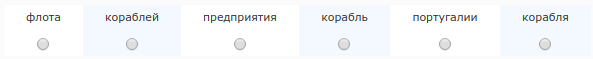
\includegraphics[width=\columnwidth]{604.png}
        \caption{non-lemmatized, not detected}
        \label{fig:word-intrusion:nonlem:fail}
    \end{subfigure}
    \begin{subfigure}[b]{0.77\columnwidth}
        
\includegraphics[width=\columnwidth]{608.png}
        \caption{lemmatized, detected}
        \label{fig:word-intrusion:lem:succ}
    \end{subfigure}
    \begin{subfigure}[b]{0.95\columnwidth}
        
\includegraphics[width=\columnwidth]{610.png}
        \caption{non-lemmatized, detected}
        \label{fig:word-intrusion:nonlem:succ}
    \end{subfigure}
    \caption{Examples of word intrusion interface on
        filtered-vocabulary whole documents.  The intruders in the
        first two examples were not detected by the annotator whereas
        those in the last two examples were detected.
    }
    \label{fig:word-intrusion}
\end{figure}

\todo{explain all those Russian words in figure/table, or remove}

If the model is interpretable, the $m$ words from a topic will be
internally coherent whereas the intruder word is likely to stand out.
Thus a model's interpretability can be quantified by the fraction
of topics for which the expert correctly identifies the intruder.  We
call this value the \emph{detection rate}:
\begin{align*}
    \DR = \frac{1}{K} \sum_{k=1}^K \dirac{i_k}{\omega_k}
\end{align*}
where $K$ is the number of topics in the model, $i_k$ is the index
of the intruder in the randomized word list generated from topic $k$,
and $\omega_k$ is the index of the word the expert identified as the
intruder.  We note this is just the mean (over topics) of the
\emph{model precision} metric from prior work~\cite{chang2009}
when one expert is used instead of several non-experts.

Our corpus consists of Russian Wikipedia pages
\todo{give details of data collection, lemmatizer}.
In constructing the lemmatized view of the corpus, when the lemmatizer
does not recognize a word we back off to the word itself.
\todo{give num/frac unknown};

We consider two preprocessing schemes to account for stop words and
other high-frequency terms in the corpus.  First, we compute the
vocabulary as the top 10,000 words by document frequency,\footnote{
    Due to minor implementation concerns the lemmatized and
    non-lemmatized vocabularies consist of the top 9387 and 9531 words
    (respectively) by document frequency.
}
separately for the lemmatized and non-lemmatized data, and
specify an asymmetric prior on each document's topic proportions
$\vtheta$.
We refer to this preprocessing scheme
as the \emph{unfiltered vocabulary}.  The second modeling scheme we
consider uses a vocabulary with high-frequency words filtered out and a
uniform prior on the document-wise topic proportions.
Specifically, a 10,000 word vocabulary is formed from the
lemmatized data by removing the top 100 words by document frequency
over the corpus and taking the next 10,000.  To determine the
non-lemmatized vocabulary, we map the filtered lemmatized
vocabulary onto all word forms that produce one of those lemmas in
the data.  Finally, observing that some of the uninformative
high-frequency words reappear in this projection, we remove any
of the top 100 words from the lemmatized and non-lemmatized corpora
from this list, producing a non-lemmatized vocabulary of 72,641 words.
While the relatively large size of this vocabulary makes the model
slower to learn, we do not believe it impacts the results negatively;
our priority is retaining the information captured by the lemmatized
vocabulary in order to provide a fair comparison.
In the filtered-vocabulary scheme we set $\alpha$ to be a uniform
vector, again with sum 5.

In addition to exploring different choices of vocabulary, we also
consider truncating the documents to their first 50 tokens.\footnote{
    Because the vocabulary does not contain rare words, the number of
    tokens in a document seen by the model is generally less than 50.
}
This augmentation simulates data sparsity by reducing the amount of
content-bearing signal in each document, so we might expect the
truncated documents to more greatly benefit from lemmatization (which
can be cast as a dimensionality reduction method).

We learn LDA by stochastic variational
inference~\cite{hoffman2013}, initializing the models randomly and
using fixed priors.\footnote{
    In preliminary experiments Gibbs
    sampling with hyper-parameter optimization was not found to improve
    interpretability.
}
We specify $K = 100$ topics to all models.
Uniform priors with $\eta_v = 0.1$ and
$\alpha_k = 5 / K$ were given to models on
filtered vocabularies; non-uniform priors with
$\eta_v = 0.1$, $\alpha_1 = 5$, and $\alpha_k = 5 / (K-1)$
for $k > 1$
were given to models on unfiltered vocabularies.
The local prior parameters $\valpha$ are informed by mean
document word usage and document length; in particular, we
believe approximately 50\% of the word tokens in the corpus are
uninformative to a topic model.

The detection rate for all four configurations (filtered or unfiltered
vocabulary and whole or truncated documents), and the
p-values for one-sided detection rate differences (testing our
hypothesis that the lemmatized models yield higher detection rates than
the non-lemmatized models), are reported in
Table~\ref{tab:detection-rate}.  Word intrusion performance benefits
significantly from lemmatization on a filtered vocabulary.  On an
unfiltered vocabulary with a prior designed to reduce topic pollution
by stop words lemmatization renders no significant improvement.
Additionally, on length-truncated documents, neither the filtered nor
unfiltered models are benefitted by lemmatization.

\begin{table}
    \begin{tabular}{l|rr|r}
        experiment            & non-lem $\DR$ &     lem $\DR$ &       p-value \\\hline
        whole                 &          0.54 &          0.52 &          0.61 \\
        \textbf{whole + filt} & \textbf{0.50} & \textbf{0.65} & \textbf{0.02} \\
        trunc                 &          0.37 &          0.37 &          0.50 \\
        trunc + filt          &          0.43 &          0.47 &          0.28 \\
    \end{tabular}
    \caption{Detection rate ($\DR$) for the non-lemmatized and
        lemmatized models
        and p-values for the one-sided detection rate difference tests.
        (trunc denotes truncated documents; filt denotes a filtered
        vocabulary.)
        The detection rate benefits significantly from lemmatization on
        a filtered vocabulary (highlighted in bold).}
    \label{tab:detection-rate}
\end{table}

\todo{explain results, in particular look at configurations other than
    the significant one, and look at how a given document is
    represented in various models}


\section{Discussion}\label{sec:discussion}

\todo{flesh out discussion}

Our results illustrate not only the importance of morphological
variation in topic models on Russian language data, but also the
dependence of conclusions derived from topic models on specific
preprocessing choices such as the handling of stop words.  One
interesting direction for future work would be the application of more
flexible models like SAGE~\cite{eisenstein2011} or the
nHDP~\cite{paisley2015} to explicitly account for such nuisance
variables in the model.

The insignificance of the truncated-document
results may be due to low baseline interpretability; if so, future work
on less morphologically-rich languages like English should take care
to design experiments that are sufficiently powerful and incisive to
separate the impacts of morphology from other sources of variability.


\section{Conclusion}\label{sec:conclusion}

We have demonstrated the impact of lemmatization as a preprocessing
step to LDA on Wikipedia articles in Russian.  In particular, we have
shown that lemmatization significantly improves interpretability, as
measured by word intrusion performance, under certain other
preprocessing conditions.  This constitutes a first step toward a full
understanding of the role of morphology in topic modeling, an issue
that has long been hinted in the applications of topic models but
never studied itself.


\bibliographystyle{acl2016}
\bibliography{russian}

\end{document}
